% ============================================================
%  XConn Technologies 产品介绍 —— Beamer 演示文稿
%  编译引擎：XeLaTeX（支持中文）
%  编译命令：xelatex xconn_presentation.tex
%  屏幕比例：16:9（宽屏）
% ============================================================

\documentclass[UTF8,9pt,aspectratio=169]{beamer}

% ============================================================
%  中文与字体设置
% ============================================================
\usepackage{xeCJK}
\setCJKmainfont{Songti SC}
\setCJKsansfont{Heiti SC}
\setCJKmonofont{STFangsong}

% ============================================================
%  主题与配色
% ============================================================
\usetheme{Darmstadt}
\usecolortheme{whale}
\usefonttheme{professionalfonts}

% ============================================================
%  常用宏包
% ============================================================
\usepackage{graphicx}
\usepackage{tikz}
\usetikzlibrary{positioning,calc,shapes.geometric,arrows.meta,backgrounds,fit,chains}
\usepackage{booktabs}
\usepackage{tabularx}
\usepackage{multirow}
\usepackage{array}
\usepackage[table]{xcolor}
\usepackage{amsmath,amssymb}
\usepackage{mathtools}
\usepackage{listings}
\usepackage{hyperref}
\usepackage{bookmark}

% ============================================================
%  文档信息
% ============================================================
\title[XConn 产品]{XConn Technologies —— CXL / PCIe 交换机芯片产品}

\author{}
\date{\today}
\institute{}

% ============================================================
%  正文
% ============================================================
\begin{document}

% ============================================================
%  标题页
% ============================================================
\begin{frame}
    \titlepage
    \vspace{0.3cm}
    \begin{center}
        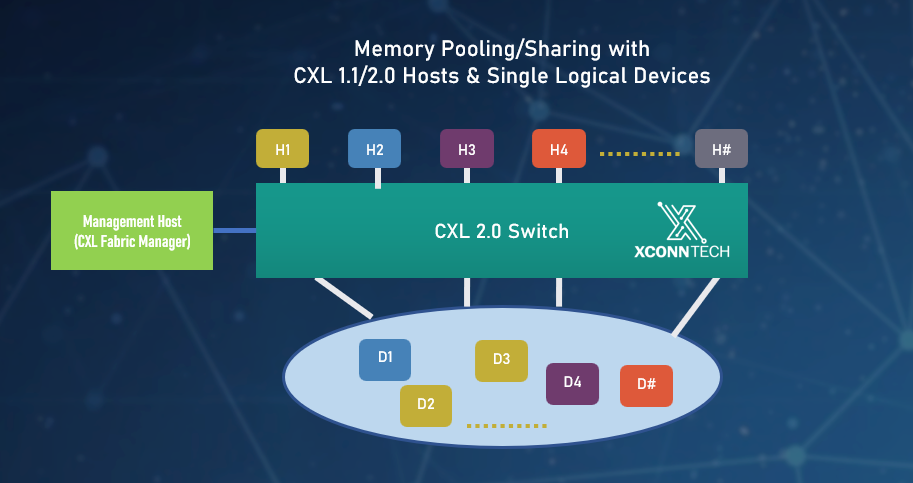
\includegraphics[width=0.35\textwidth]{figs/xconn_chip.png}
    \end{center}
    {\footnotesize \hfill 现已并入 Marvell (2026)}
\end{frame}

% ============================================================
%  XC50256 CXL 2.0 Switch Chip
% ============================================================
\section{XC50256 CXL 2.0 Switch Chip}

\begin{frame}{XC50256 CXL 2.0 Switch Chip}{世界首款 CXL 2.0 / PCIe Gen 5.0 交换机芯片}
    \begin{columns}[T]
        \begin{column}{0.42\textwidth}
            \begin{figure}
                \centering
                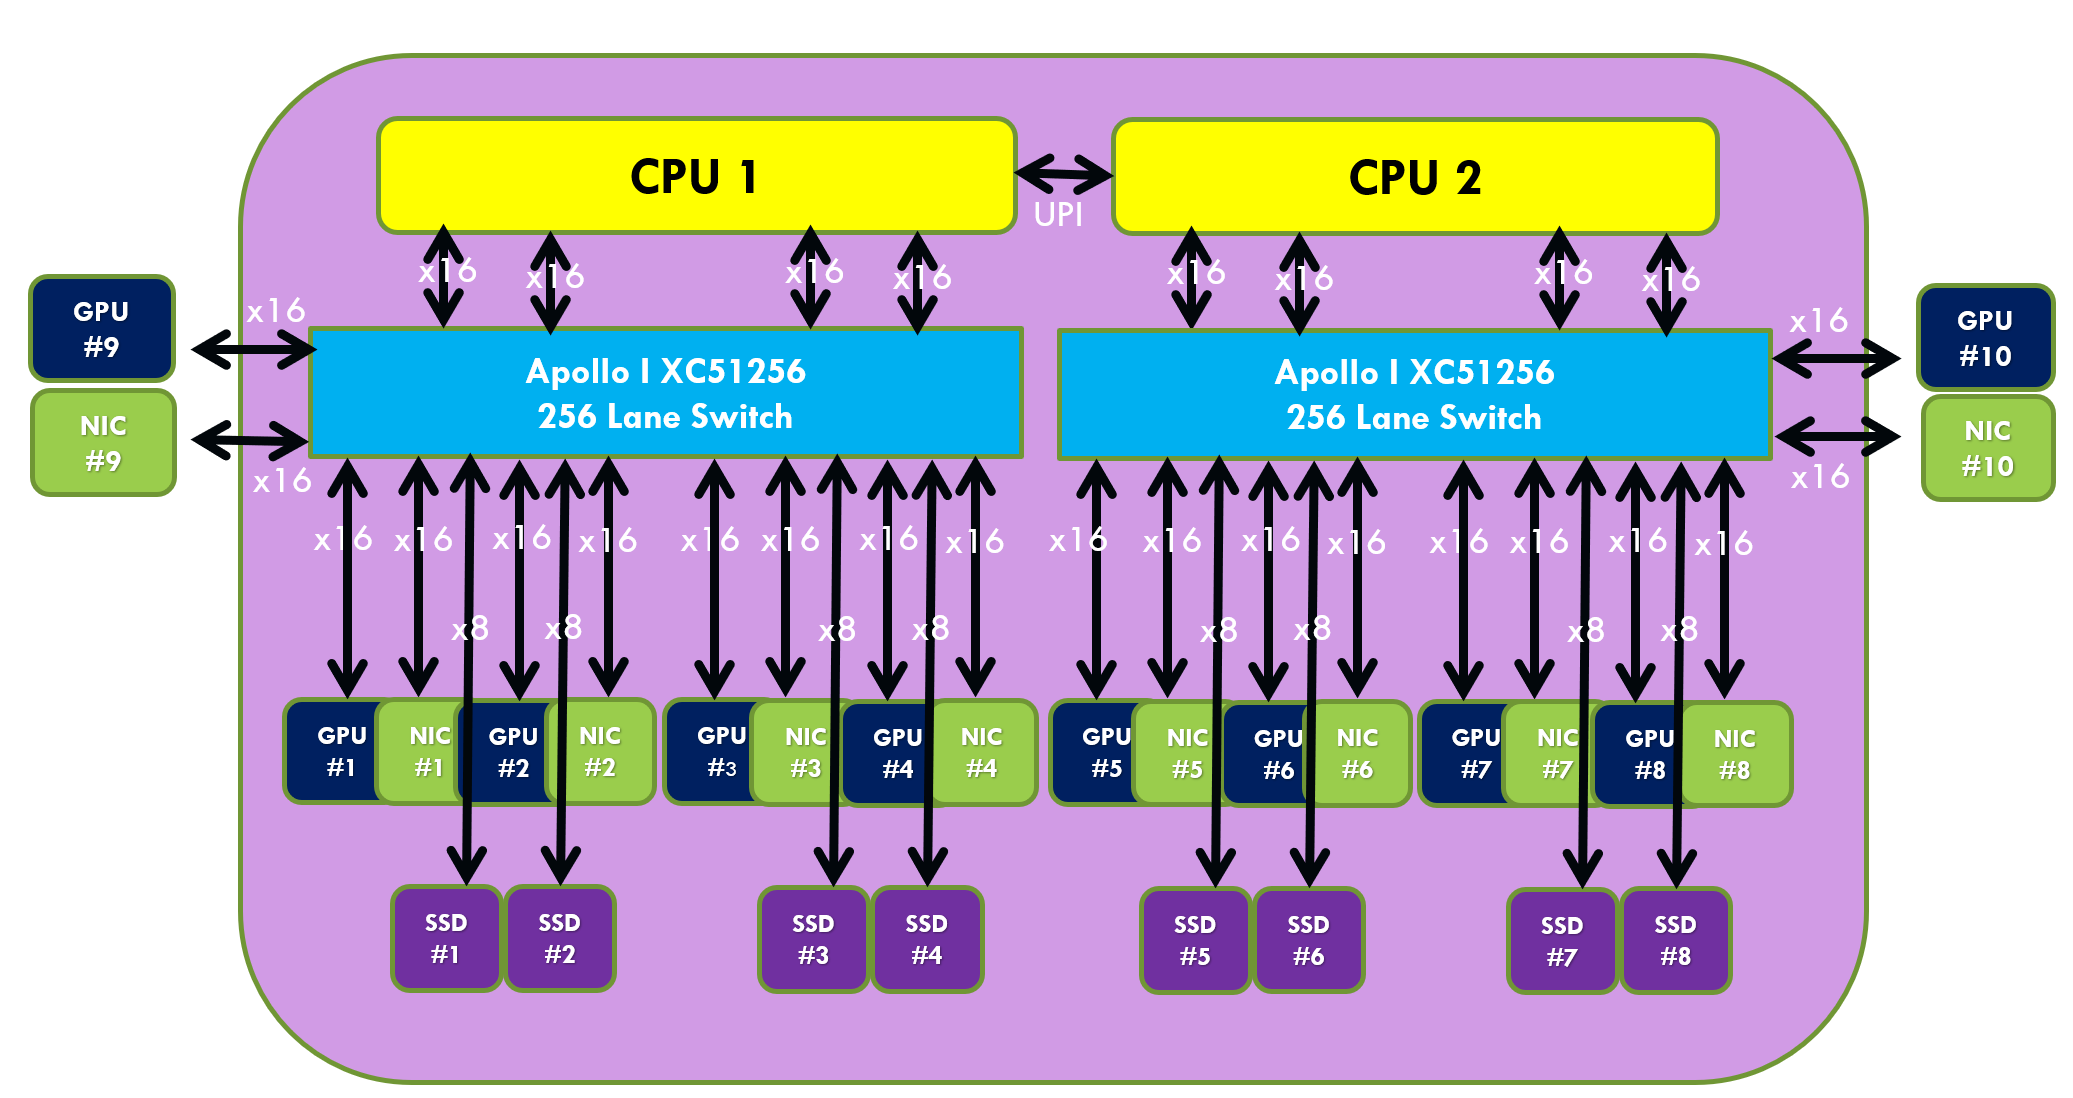
\includegraphics[width=\textwidth]{figs/xconn_km_diagram.png}
                \caption{KM 框图}
            \end{figure}
        \end{column}
        \begin{column}{0.55\textwidth}
            \begin{itemize}
                \item 完全兼容 \textbf{CXL 2.0 / 1.1} 与 \textbf{PCIe Gen 5.0}
                \item 支持 \textbf{CXL.io、CXL.mem、CXL.cache}
                \item CXL Fabric Manager 接口，支持 \textbf{MLD}（Multi-Logical Device）
                \item 多虚拟 CXL 交换机（\textbf{VCS}）
                \item 支持 \textbf{CXL Type 2 / Type 3} 内存设备
                \item 总计 \textbf{32 端口}（含 Bifurcation），\textbf{256 Lane}
                \item 交换容量 \textbf{2,048\,GB/s}
                \item 业内最低端口到端口延迟
                \item 低功耗/端口，减小 PCB 面积，降低 TCO
                \item 完整 RAS 支持：ECC/Parity、DPC、Hot-Plug、Data Poisoning
            \end{itemize}
        \end{column}
    \end{columns}

    \vspace{0.2cm}
    {\footnotesize 参考链接：\href{https://www.xconn-tech.com/products}{XConn Technologies —— Products}}
\end{frame}

% ============================================================
%  XC51256 PCIe Gen 5.0 Switch Chip
% ============================================================
\section{XC51256 PCIe Gen 5.0 Switch Chip}

\begin{frame}{XC51256 PCIe Gen 5.0 Switch Chip}{纯 PCIe 交换机芯片}
    \begin{columns}[T]
        \begin{column}{0.55\textwidth}
            \begin{itemize}
                \item 完全兼容 \textbf{PCIe Gen 5.0} 规范
                \item 业内 \textbf{最低延迟} PCIe Gen 5.0 交换机
                \item 业界 \textbf{最大 Lane 数} PCIe 交换机：\textbf{256 Lane}
                \item x8 / x16 端口 Bifurcation，最多 \textbf{32 端口}
                \item 支持 \textbf{虚拟交换机}、\textbf{非透明桥}（NTB）、\textbf{多主机 IO 共享}
                \item 支持 Hot-Plug、Hot-Add、Hot-Remove、Surprise-Plug
                \item 内嵌逻辑分析仪（\textbf{ELA}）+ Debug GUI 诊断
                \item 接口：I2C、SPI、UART、GPIO、JTAG、SRIS/SRNS
            \end{itemize}
        \end{column}
        \begin{column}{0.42\textwidth}
            \begin{figure}
                \centering
                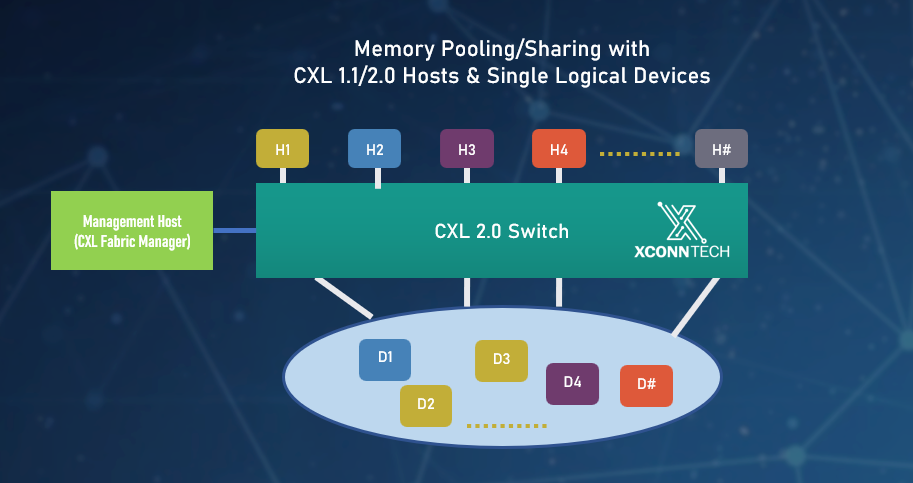
\includegraphics[width=\textwidth]{figs/xconn_chip.png}
                \caption{XC51256 产品图}
            \end{figure}
        \end{column}
    \end{columns}

    \vspace{0.2cm}
    {\footnotesize 参考链接：\href{https://www.xconn-tech.com/products}{XConn Technologies —— Products}}
\end{frame}

\end{document}
